% RESULTADOS-------------------------------------------------------------------

\chapter{ANÁLISE E RESULTADOS}
\label{chap:resultados}

Este capítulo tem o propósito de demonstrar e fazer a análise dos resultados obtidos no trabalho.
Serão analisados os seguintes resultados:

\begin{itemize}
    \vspace{0.5em}
    \item Reconstrução dos cenários virtuais;
    \item Reconstrução dos cenários reais;
    \item Resultados dos contextos virtuais;
    \item Resultados dos contextos reais;
    \item Desempenho dos algoritmos de cálculo de volume e superfície.
    \item Comparação entre reconstrução em simulação e no experimento;
\end{itemize}
\vspace{1em}

Os resultados da reconstrução de ambas coletas serão avaliados de duas formas: a primeira será a avaliação individual de cada cenário, enquanto que a segunda será a avaliação dos contextos.
Além de fazer a análise da simulação separada da análise em campo, serão comparados os resultados obtidos nos cenários e contextos virtuais com os reais.
Outra análise que será realizada é em relação ao desempenho dos algoritmos de cálculo de volume e superfície, pois esses influenciam diretamente na taxa de acerto da reconstrução.


\section{Simulação virtual}

\subsection{Avaliação da reconstrução dos cenários}
\label{sec:avaliacao_cenarios}

Os resultados da reconstrução dos cenários, apresentados na Seção \ref{sec:simulation}, estão retratados na Tabela  \ref{tab:tabela_result_cenarios_sup}, na Tabela \ref{tab:tabela_result_cenarios_vol} e na Figura \ref{fig:recontrucao_virtual}.
Observa-se que nenhum resultado obteve 100\% na taxa de acerto, porque isso é praticamente uma utopia.

A Tabela \ref{tab:tabela_result_cenarios_sup} mostra o resultado da reconstrução da superfície através da diferença entre a área esperada e a área calculada pelo algoritmo.
A avaliação do desempenho da reconstrução em 3D é ditada pela taxa de acerto destes dados.
A superfície foi maior do que o esperado nos cenários A e B porque os pontos da nuvem não ficarão alinhados em um único plano e isso faz com que a triangulação fique desparelha, como se a parede reconstruída parecesse "amassada".
No cenário C o resultado foi menor do que o esperado, pois na coleta quando o robô estava se aproximando ao solo, os sinais com maior intensidade estava vindo do solo e não da rampa, problema causado pela ambiguidade (Seção \ref{sec:imagem_acustica}).

\begin{table}[H]
    \centering
    \caption{Resultados obtidos do cálculo de superfície de cada cenário.}
    \begin{tabular}{@{}ccccc@{}}
        \toprule
        \textbf{Cenário} & \textbf{Superfície esperada} & \textbf{Superfície calculada} & \textbf{Diferença} & \textbf{Taxa de acerto} \\ \midrule
        \textbf{A} & 1.200,00 uc$^2$ & 1.273,57 uc$^2$ & 73,57 uc$^2$ & 93,87\% \\
        \textbf{B} & 1.200,00 uc$^2$ & 1.280,02 uc$^2$ & 80,02 uc$^2$ & 93,33\% \\
        \textbf{C} & 1.697,06 uc$^2$ & 1.591,02 uc$^2$ & 106,04 uc$^2$ & 93,75\% \\ \bottomrule
    \end{tabular}
    \label{tab:tabela_result_cenarios_sup}
\end{table}

A Tabela \ref{tab:tabela_result_cenarios_vol} mostra os resultados de cada cenário em relação ao volume.
Os resultados do cálculo de volume não são diferentes em relação ao cálculo de superfície, portantos os motivos são os mesmos.

A Figura \ref{fig:recontrucao_virtual} mostra o processo de reconstrução dos três cenários. 
A primeira imagem mostra a criação da nuvem de pontos após a etapa de pré-processamento.
A segunda imagem mostra a nuvem de pontos após a etapa de filtragem.
Na terceira imagem, a reconstrução da superfície.
A última imagem exibe o volume gerado a partir da superfície.

\begin{table}[H]
    \centering
    \caption{Resultados obtidos do cálculo de volume de cada cenário.}
    \begin{tabular}{@{}ccccc@{}}
        \toprule
        \textbf{Cenário} & \textbf{Volume esperado} & \textbf{Volume calculado} & \textbf{Diferença} & \textbf{Taxa de acerto} \\ \midrule
        \textbf{A} & 36.000,00 uc$^3$ & 37.862,51 uc$^3$ & 1.862,51 uc$^3$ & 94,83\% \\
        \textbf{B} & 1.200,00 uc$^3$ & 1.251,83 uc$^3$ & 51,83 uc$^3$ & 95,68\% \\
        \textbf{C} & 18.000,00 uc$^3$ & 16.830.45 uc$^3$ & 1.169,54 uc$^3$ & 93,50\% \\ \bottomrule
    \end{tabular}
    \label{tab:tabela_result_cenarios_vol}
\end{table}

\begin{figure}[H]
    \centering
    \caption{Reconstrução dos cenários em simulação virtual.}
    \label{fig:recontrucao_virtual}
    \begin{subfigure}[t]{\textwidth}
        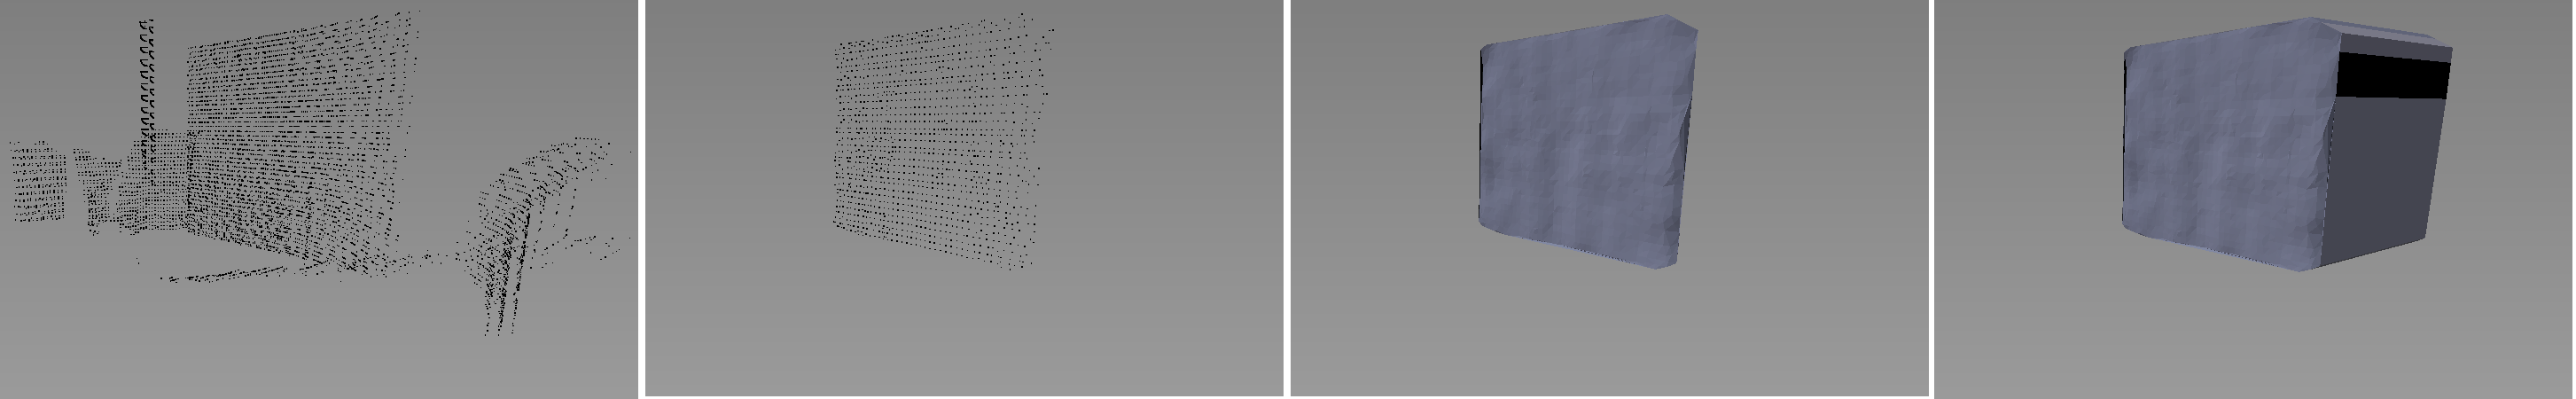
\includegraphics[width=\textwidth]{dados/figuras/wall3.png}
        \caption{Cenário A}
    \end{subfigure}
    \begin{subfigure}[t]{\textwidth}
        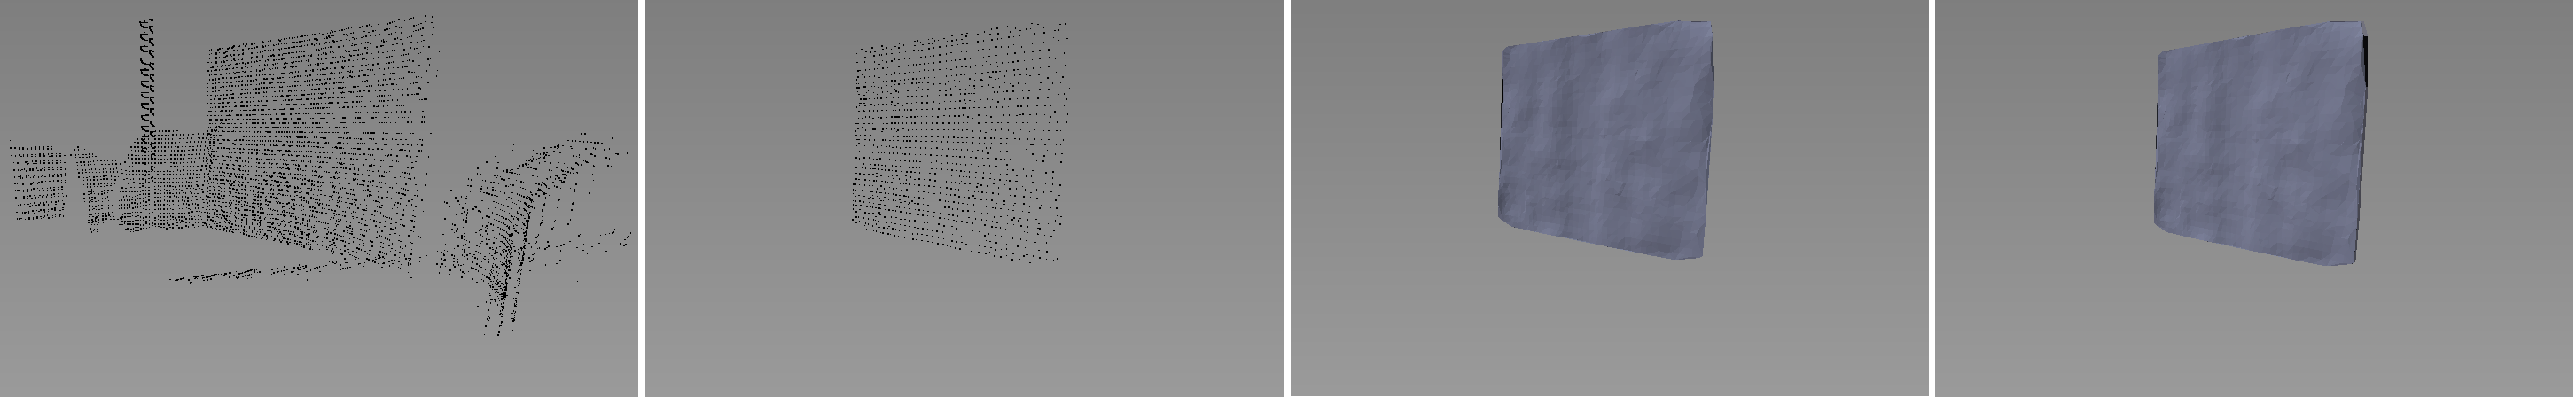
\includegraphics[width=\textwidth]{dados/figuras/wall.png}
        \caption{Cenário B}
    \end{subfigure}
    \begin{subfigure}[t]{\textwidth}
        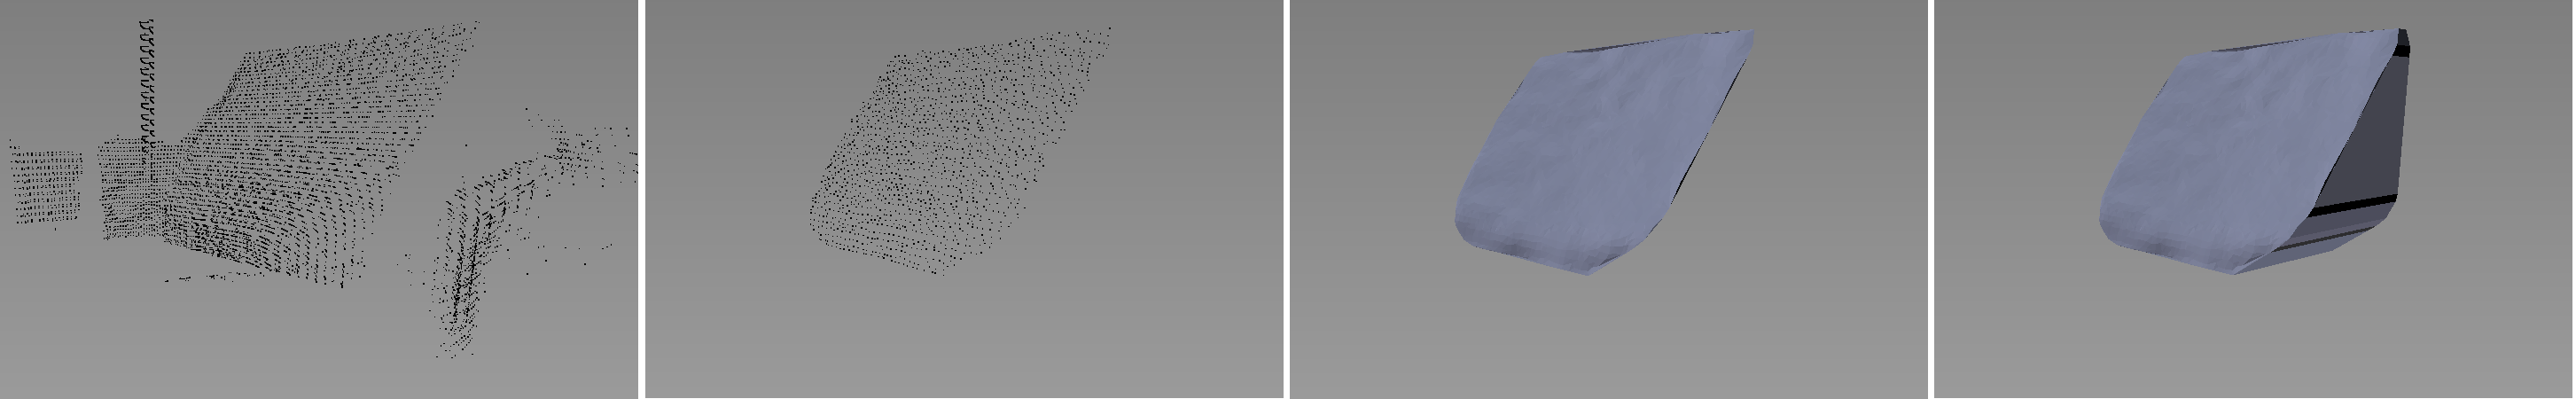
\includegraphics[width=\textwidth]{dados/figuras/declined.png}
        \caption{Cenário C}
    \end{subfigure}
\end{figure}

\subsection{Avaliação dos contextos}
\label{sec:avaliacao_contextos}

Essa seção descreve os resultados obtidos nas comparações de cenários, os chamados contextos (os contextos foram descritos na Seção \ref{sec:simulation}).
No primeiro contexto (AB), o volume calculado foi quase igual ao esperado, porém não foi melhor por causa de pequenos ruídos remanescentes e da própria reconstrução.
O segundo contexto (AC) foi obtido um resultado mediano, onde o principal motivo foi por conta do volume obtido na reconstrução do cenário C, que já foi explicado na seção anterior. 

\begin{table}[H]
    \centering
    \caption{Resultados obtidos do cálculo de comparação de volume.}
    \begin{tabular}{ccccc}
        \toprule
        \textbf{Contexto} & \textbf{Volume esperado} & \textbf{Volume calculado} & \textbf{Diferença} & \textbf{Taxa de acerto} \\ \midrule
        \textbf{AB} & 6.000 uc$^3$ & 6.288,77 uc$^3$ & 288,77 uc$^3$ & 95,41\% \\
        \textbf{AC} & 18.000 uc$^3$ & 11.594,48 uc$^3$ & 6.405,52 uc$^3$ & 64,41\% \\ \bottomrule
    \end{tabular}
    \label{tab:tabela_resultados_contextos}
\end{table}


\section{In loco}
